\begin{figure}[H]
	\center{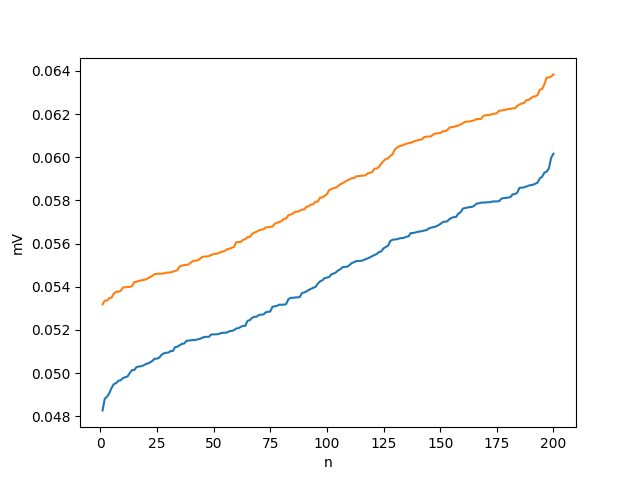
\includegraphics[width=0.5\linewidth]{images/data.png}}
	\caption{Результаты измерений величины токов.}
	\label{ris:image2}
\end{figure}

\begin{figure}[H]
	\center{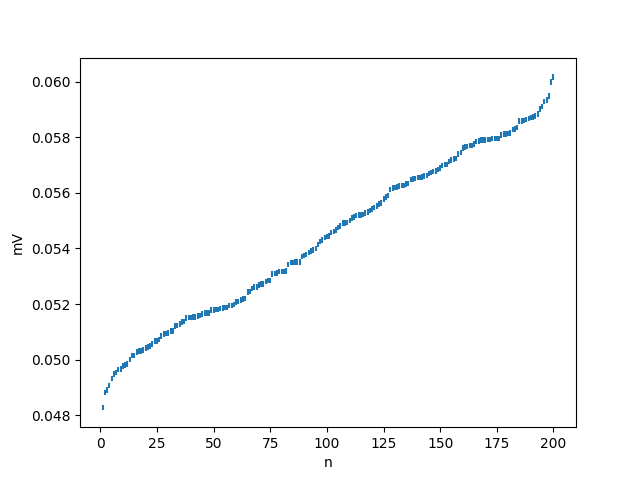
\includegraphics[width=0.5\linewidth]{images/data_and_intervals1.png}}
	\caption{Интервальное представление данных для выборки 1.}
	\label{ris:image2}
\end{figure}

\begin{figure}[H]
	\center{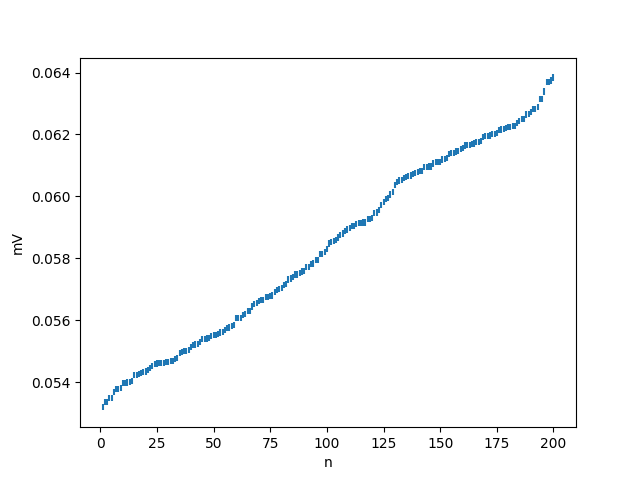
\includegraphics[width=0.5\linewidth]{images/data_and_intervals2.png}}
	\caption{Интервальное представление данных для выборки 2.}
	\label{ris:image2}
\end{figure}

\begin{figure}[H]
	\center{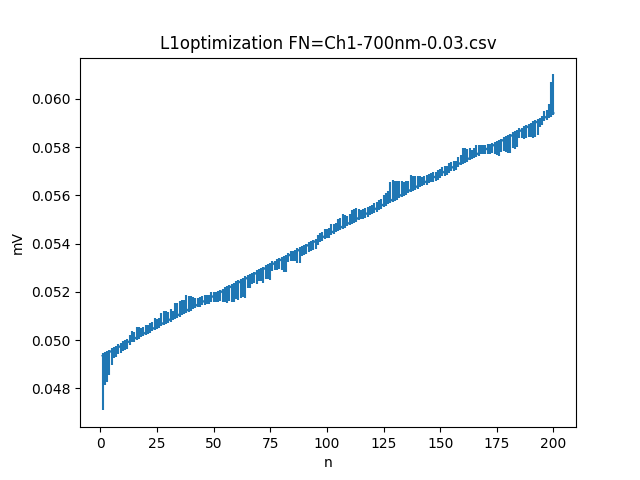
\includegraphics[width=0.5\linewidth]{images/di1.png}}
	\caption{Линейная модель дрейфа данных из выборки 1.}
	\label{ris:image1}
\end{figure}

\begin{figure}[H]
	\center{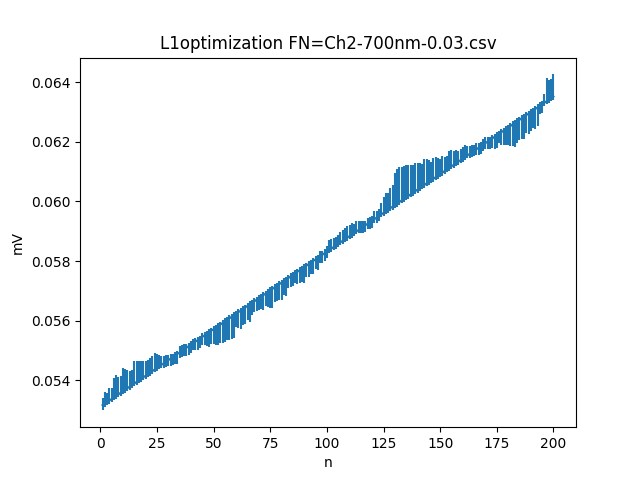
\includegraphics[width=0.5\linewidth]{images/di2.png}}
	\caption{Линейная модель дрейфа данных из выборки 2.}
	\label{ris:image1}
\end{figure}

\begin{figure}[H]
	\center{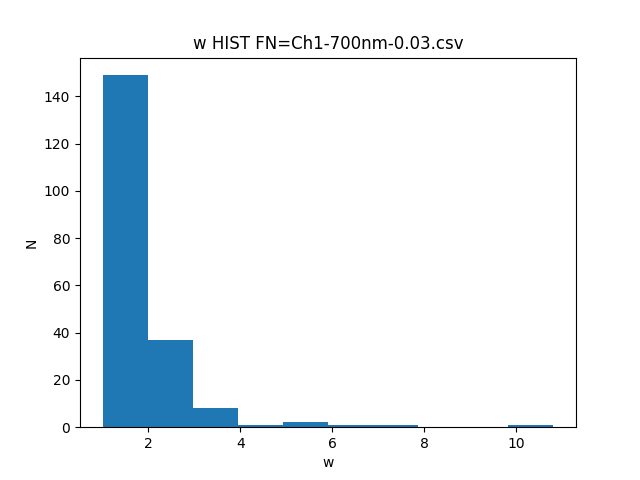
\includegraphics[width=0.5\linewidth]{images/hist1.png}}
	\caption{Гистограмма значений множителей коррекции $w$ из выборки 1.}
	\label{ris:hist1}
\end{figure}

\begin{figure}[H]
	\center{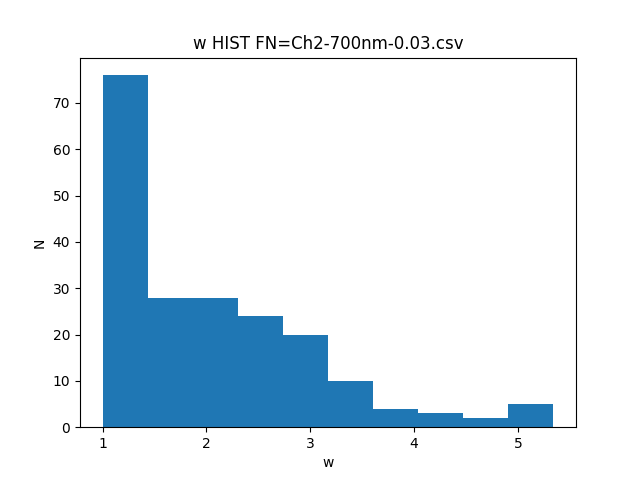
\includegraphics[width=0.5\linewidth]{images/hist2.png}}
	\caption{Гистограмма значений множителей коррекции $w$ из выборки 2.}
	\label{ris:hist2}
\end{figure}

\begin{figure}[H]
	\center{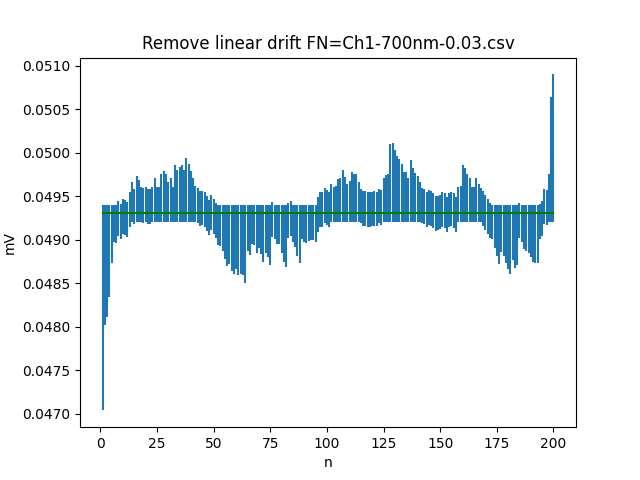
\includegraphics[width=0.5\linewidth]{images/interval_new1.png}}
	\caption{Скорректированная модель данных из выборки 1.}
	\label{ris:hist2}
\end{figure}

\begin{figure}[H]
	\center{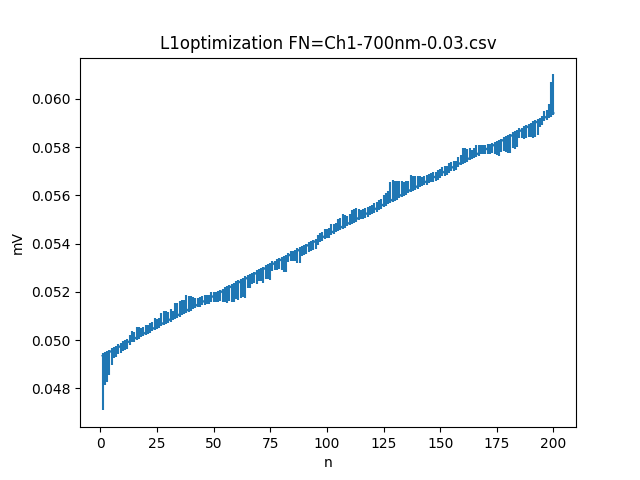
\includegraphics[width=0.5\linewidth]{images/di1.png}}
	\caption{Линейная модель дрейфа данных из выборки 1.}
	\label{ris:image1}
\end{figure}

\begin{figure}[H]
	\center{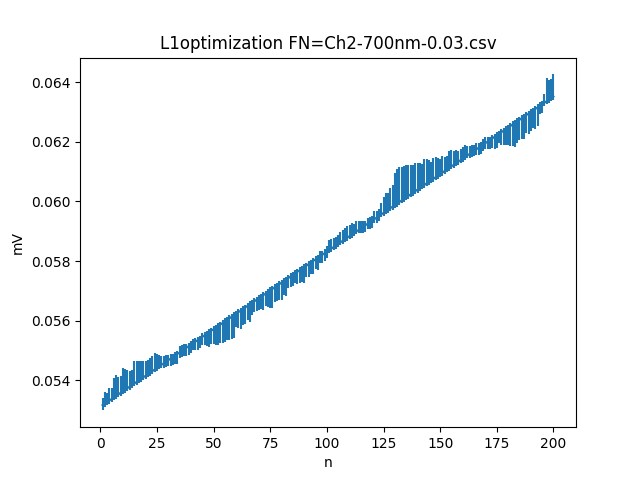
\includegraphics[width=0.5\linewidth]{images/di2.png}}
	\caption{Линейная модель дрейфа данных из выборки 2.}
	\label{ris:image1}
\end{figure}

\begin{figure}[H]
	\center{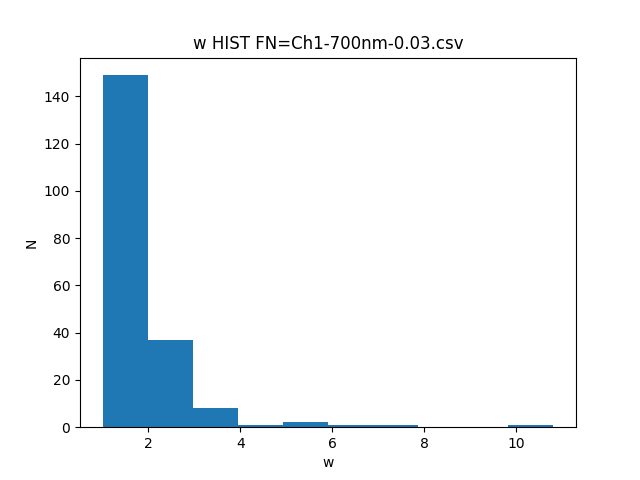
\includegraphics[width=0.5\linewidth]{images/hist1.png}}
	\caption{Гистограмма значений множителей коррекции $w$ из выборки 1.}
	\label{ris:hist1}
\end{figure}

\begin{figure}[H]
	\center{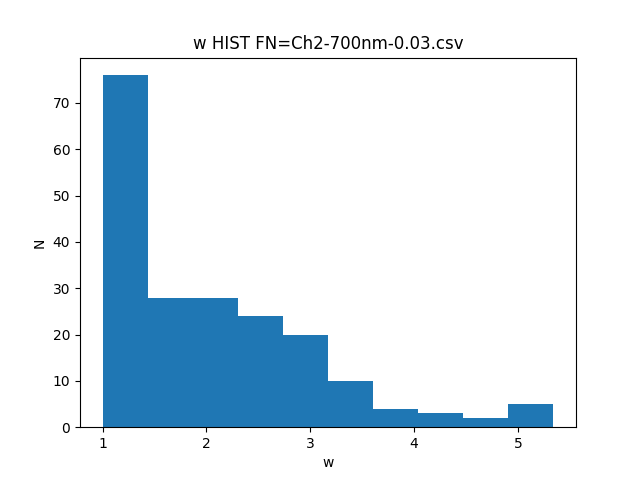
\includegraphics[width=0.5\linewidth]{images/hist2.png}}
	\caption{Гистограмма значений множителей коррекции $w$ из выборки 2.}
	\label{ris:hist2}
\end{figure}

\begin{figure}[H]
	\center{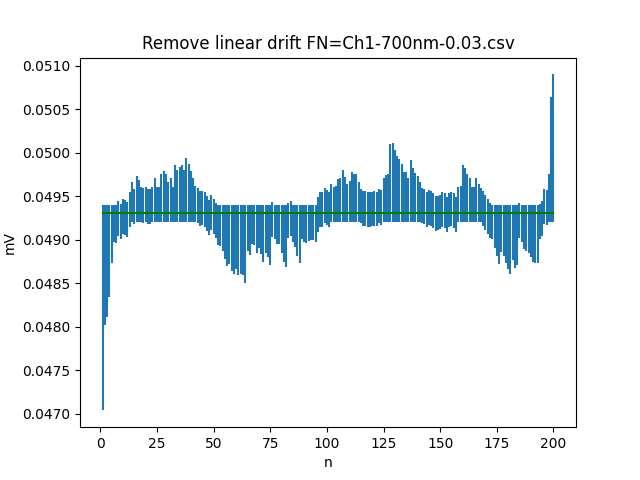
\includegraphics[width=0.5\linewidth]{images/interval_new1.png}}
	\caption{Скорректированная модель данных из выборки 1.}
	\label{ris:hist2}
\end{figure}

\begin{figure}[H]
	\center{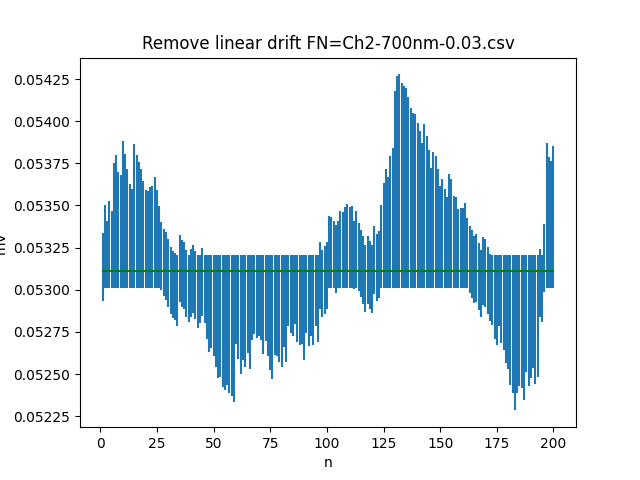
\includegraphics[width=0.5\linewidth]{images/interval_new2.png}}
	\caption{Скорректированная модель данных из выборки 2.}
	\label{ris:hist2}
\end{figure}

\begin{figure}[H]
	\center{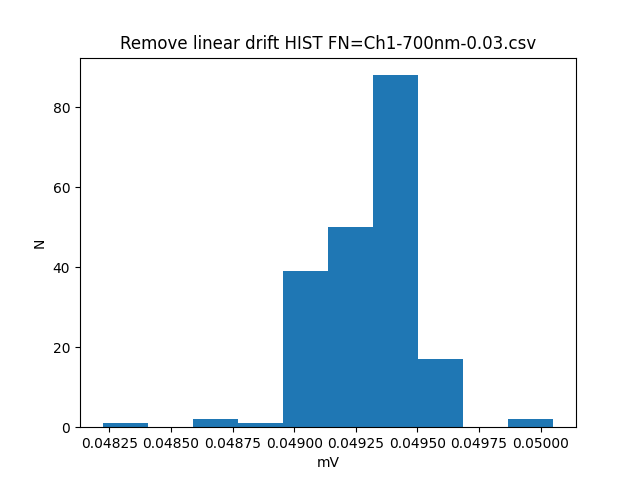
\includegraphics[width=0.5\linewidth]{images/hist_interval1.png}}
	\caption{Гистограмма скорректированной модели данных из выборки 1.}
	\label{ris:hist2}
\end{figure}

\begin{figure}[H]
	\center{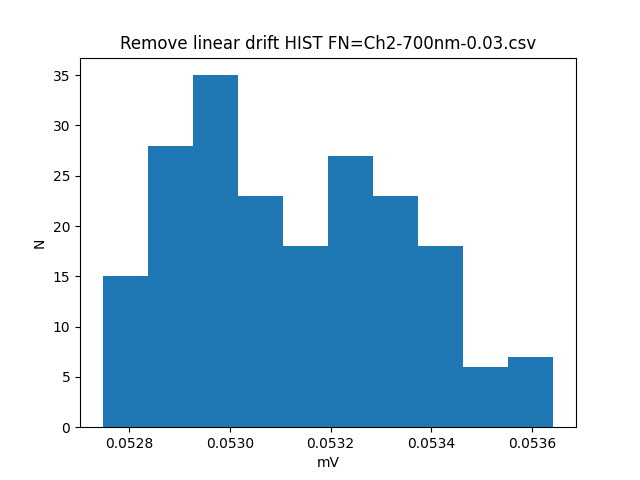
\includegraphics[width=0.5\linewidth]{images/hist_interval2.png}}
	\caption{Гистограмма скорректированной модели данных из выборки 2.}
	\label{ris:hist2}
\end{figure}

\begin{figure}[H]
	\center{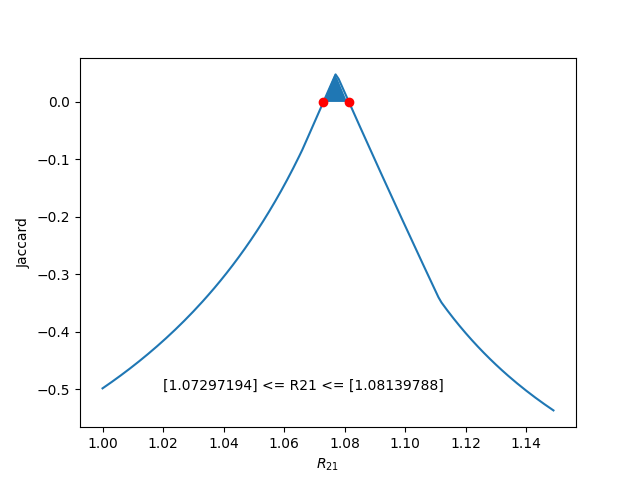
\includegraphics[width=0.5\linewidth]{images/jakkar.png}}
	\caption{Зависимость коэффициента Жаккара от $R_{21}$}
	\label{ris:hist2}
\end{figure}

\begin{figure}[H]
	\center{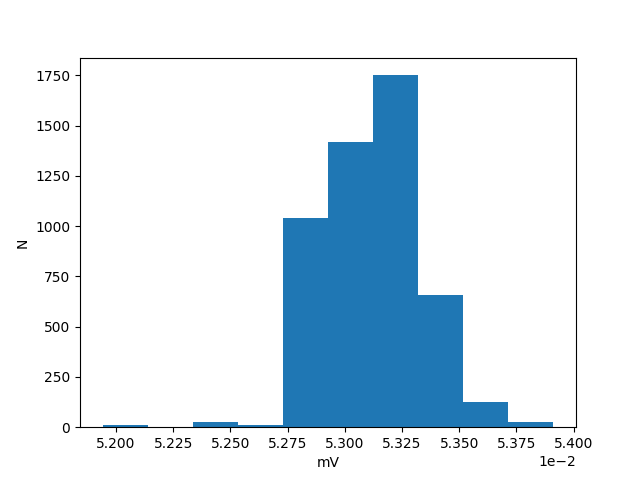
\includegraphics[width=0.5\linewidth]{images/jakkar_combined_hist.png}}
	\caption{Гистограмма объединенной выборки при $R_{21}$}
	\label{ris:hist2}
\end{figure}
